\chapter{Versuch 2}
\label{chap:VERSUCH_2}

\section{Fragestellung, Messprinzip, Aufbau, Messmittel}
\label{chap:VERSUCH_2_FRAGESTELLUNG}




Bei Versuch 2 ging es um die Modellierung der Kennlinie durch lineare Regression. 

\subsection*{Fragestellung}

	Da es sich bei diesem Abstandssensor um einen mit nicht linearer Funktion handelt, sondern um eine Potenzfunktion:
	\begin{equation*}
  	y = x^a
\end{equation*}
	muss diese erst logarithmiert werden. Im nach hinein muss  die Ausgleichsgerade mit Hilfe der linearen Regression erzeugt werden.


\section{Messwerte}
\label{chap:VERSUCH_2_MESSWERTE}
\begin{center}
\begin{tabular}{|c|c|}
\hline 
Abstand (cm) & Spannung (Volt) \\ 
\hline 
10 & 1,363 \\ 
\hline 
13 & 1,212 \\ 
\hline 
16 & 1,078 \\ 
\hline 
19 & 0,973 \\ 
\hline 
22 & 0,897 \\ 
\hline 
25 & 0,0215 \\ 
\hline 
28 & 0,7653 \\ 
\hline 
31 & 0,6992 \\ 
\hline 
34 & 0,6567 \\ 
\hline 
37 & 0,6374 \\ 
\hline 
40 & 0,5986 \\ 
\hline 
43 & 0,5604 \\ 
\hline 
46 & 0,5415 \\ 
\hline 
49 & 0,5227 \\ 
\hline 
52 & 0,5228 \\ 
\hline 
55 & 0,5037 \\ 
\hline 
58 & 0,4848 \\ 
\hline 
61 & 0,4847 \\ 
\hline 
64 & 0,4846 \\ 
\hline 
67 & 0,4846 \\ 
\hline 
70 & 0,4657 \\ 
\hline 
\end{tabular} 
\captionof{table}{Messwerte von vorherigen Studenten}\label{messdatenBlatt}
\end{center}	
	
\newpage
\section{Auswertung}
\label{chap:VERSUCH_2_AUSWERTUNG}
Die Kennlinie aus den rohen Daten sieht so aus:
	\begin{center}
		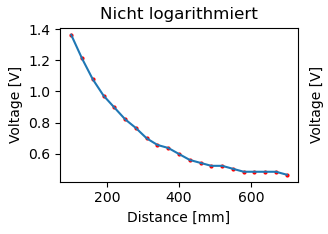
\includegraphics[scale=1.5]{media/dataV2.png}
		\captionof{figure}{Plot zu den rohen Messwerten}
	\end{center}
Dann nach der Logarithmierung der Kennlinie sieht sie folgendermaßen aus:
	\begin{center}
		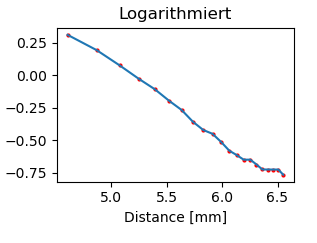
\includegraphics[scale=1]{media/linReg.png}
		\captionof{figure}{Plot zu den logarithmierten Messwerten}
	\end{center}


Jetzt muss die Ausgleichsgerade ermittelt werden nach dem Schema:
	\begin{equation}
  	y = x^a
	\end{equation}

Jedoch bevor es möglich ist \textit{a} und \textit{b} zu berechnen, muss erst der Mittelwert $\overline{x}$ ermittelt werden.\linebreak\linebreak
Dann berechnet sich \textit{a} wie folgt:
	\begin{equation}
	a = \dfrac{\sum\nolimits_{i=1}^n  (x_i - \overline{x}) * (y_i - \overline{y})  }{\sum\nolimits_{i=1}^n(x_i - \overline{x})^2}
	\end{equation}
Und \textit{b}:
	\begin{equation}
	b = \overline{y} - a * \overline{x}
	\end{equation}
	
	
	
\section{Interpretation}
\label{chap:VERSUCH_1_INTERPRETATION}
Im vorherigen Abschnitt wurden bereits \textit{a} und \textit{b} berechnet.
Daraus ergibt sich bei den gegebenen werten folgende Geradengleichung:
	\begin{equation*}
	y = -1,689x + 5,169
	\end{equation*}

Und die Lineare Regression sieht dann folgendermaßen aus:
		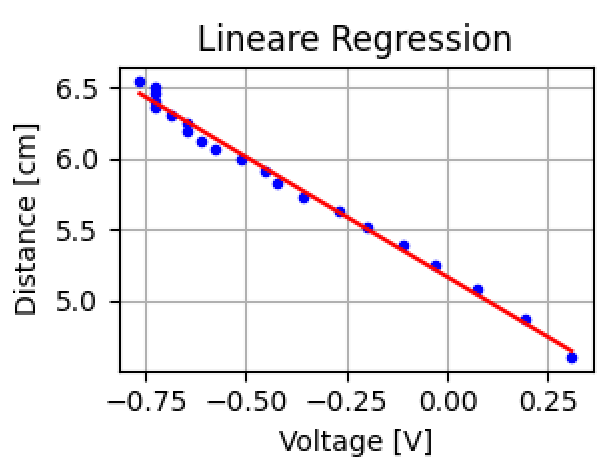
\includegraphics[scale=1]{media/linReg2.png}